We have run two different versions of the model: one that is the same as \cite{li2018deep} in order to report on the original paper's reproducibility and another version that runs the newly proposed hierarchical version of this model. Firstly, we will discuss the replicated results of the original paper. Secondly, we will discuss the results of the hierarchical model.



After training the model for 1500 epochs our model achieved 98.6\% and 98.8\% accuracy for the superprototype classification network and the subprototype classification network respectively on the MNIST test set. 

\begin{figure}[ht]
    \centering
    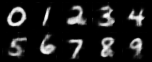
\includegraphics{img/prot1499.png}
    \caption{Superprototypes after 1500 epochs with weights set to negative identity.}
    \label{superprots}
\end{figure}

\begin{figure}[ht]
    \centering
    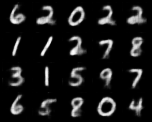
\includegraphics{img/subprot1499.png}
    \caption{Sub prototypes after 1500 epochs with learnable weights}
    \label{subprots}
\end{figure}


